%%%%%%%%%%%%%%%%%%%%%%%%%%%%%%%%%%%%%%%%%
%
% (c) 2022 by Jennifer Laaser
%
% This work is licensed under the Creative Commons Attribution-NonCommercial-ShareAlike 4.0 International License. To view a copy of this license, visit http://creativecommons.org/licenses/by-nc-sa/4.0/ or send a letter to Creative Commons, PO Box 1866, Mountain View, CA 94042, USA.
%
% The current source for these materials is accessible on Github: https://github.com/jlaaser/pogil-polymers
%
%%%%%%%%%%%%%%%%%%%%%%%%%%%%%%%%%%%%%%%%%

\renewcommand{\figpath}{content/polymphys/scattering/scattering-fundamentals/figs}
\renewcommand{\labelbase}{scattering-fundamentals}

\begin{activity}{Fundamentals of Scattering}
\label{\labelbase}

\begin{instructornotes}
	This activity introduces students to fundamental concepts related to scattering of particles and electromagnetic waves.
	
	After completing this activity, students will be able to:
	\begin{enumerate}
		\item \dots
	\end{enumerate}
	
	\subsection*{Activity summary:}
	\begin{itemize}
		\item \textbf{Activity type:} Learning Cycle
		\item \textbf{Content goals:} See above %Measuring Thermal Transitions of Polymer Materials
		\item \textbf{Process goals:} %https://pogil.org/uploads/attachments/cj54b5yts006cklx4hh758htf-process-skills-official-pogil-list-2015-original.pdf
			\begin{enumerate}
				\item Interpretation of graphical data
				\item Written and oral communication of reasoning
			\end{enumerate}
		\item \textbf{Duration:} TBD, including time for class discussion
		\item \textbf{Instructor preparation required:} none beyond knowledge of relevant content
		\item \textbf{Related textbook chapters:}
			\begin{itemize}
				\item \emph{Polymer Chemistry} (Hiemenz \& Lodge): section XX
				\item \emph{Introduction to Polymers} (Young \& Lovell): section XX
			\end{itemize}
		%\item \textbf{Instructor notes:}
		%	\begin{itemize}
		%		\item \dots
		%	\end{itemize}
	\end{itemize}
	
\end{instructornotes}



\begin{model}[Interference of Electromagnetic Waves]
	\label{\labelbase:mdl:interference}
	
	Electromagnetic waves, such as light and X-rays, consist of oscillating electric and magnetic fields propagating through space.
	The electric field, $E$, of an electromagnetic wave propagating along the $x$ axis is shown below:
	
	\vspace{6pt}
	\centerline{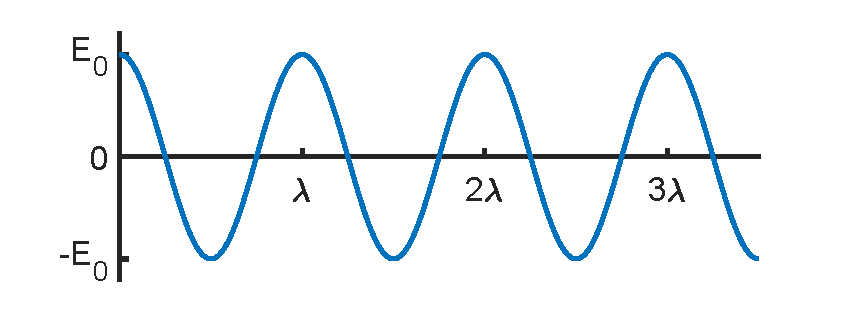
\includegraphics[width=0.6\textwidth]{\figpath/Model1_Ecosx.pdf}}
	
\end{model}


\begin{ctqs}

	\question What is the maximum value of the electric field (the \emph{amplitude} of the electric field) for the wave shown in Model \ref{\labelbase:mdl:interference}?
	
		\begin{solution}[0.25in]
			$E_0$
		\end{solution}
	
	\question At what values of $x$ is the amplitude of the wave at this maximum value?
	
		\begin{solution}[0.25in]
			0, $\lambda$, $2\lambda$, $3\lambda$
		\end{solution}
	
	\question How much does $x$ have to be increase to move from one maximum of the wave to the next?
	
		\begin{solution}[0.25in]
			$\lambda$
		\end{solution}
	
	\question Explain, in 1-2 complete sentences, why $\lambda$ is referred to as the \emph{wavelength} of the wave.
	
		\begin{solution}[1.5in]
		\end{solution}
	
	\clearpage
	\question Suppose the position of the wave is shifted to the right by $\Delta x = \frac{\lambda}{2}$.
	
		\begin{enumerate}
			\item Sketch the ``shifted'' wave on the following axes.  The original wave is shown in grey for reference.
	
				\begin{solution}[1.5in]\studentdisplay{
					\centerline{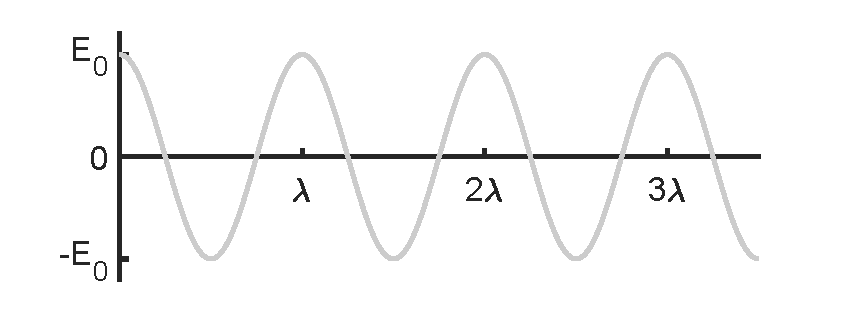
\includegraphics[width=0.6\textwidth]{\figpath/Model1_shiftedwave_blank.pdf}}
				}\instructordisplay{
					\centerline{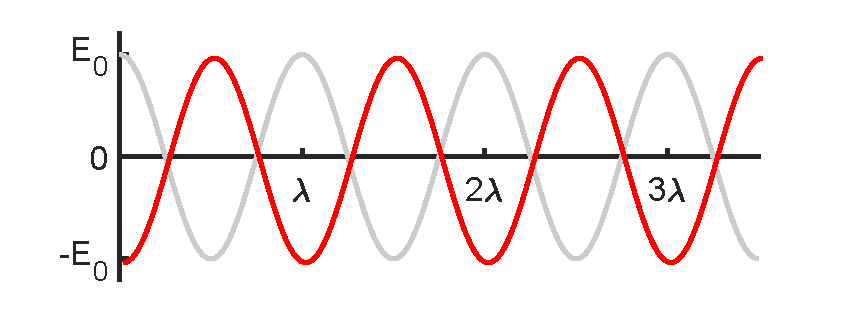
\includegraphics[width=0.6\textwidth]{\figpath/Model1_shiftedwave_solution.pdf}}
				}\end{solution}
			
			\item Does shifting the wave change change either its amplitude or its wavelength?  Briefly explain how you know.
			
				\begin{solution}[1in]
				\end{solution}
				
		\end{enumerate}

	\question Mathematically, the electric field of an electromagnetic wave propagating along the $x$ axis can be expressed as
	\begin{equation*}
		E = E_0 \cos\left( \frac{2\pi x}{\lambda} + \delta \right)
	\end{equation*}
	In this expression, which variable ($E_0$, $\lambda$, or $\delta$) controls...
	
		\begin{enumerate}
		
			\item ... the amplitude of the wave?
			
				\begin{solution}[0.25in]
					$E_0$
				\end{solution}
			
			\item ... the wavelength of the wave?
			
				\begin{solution}[0.25in]
					$\lambda$
				\end{solution}
			
			\item ... the shift in the position of the wave?
			
				\begin{solution}[0.25in]
					$\delta$
				\end{solution}
		
		\end{enumerate}
		
\end{ctqs}

\begin{infobox}
	When the amplitudes of two electromagnetic waves measured at the same position have the \emph{same} sign, we refer to those waves as \emph{in phase} with each other.
	
	When the amplitudes of two electromagnetic waves measured at the same position have \emph{different} signs, we refer to those waves as \emph{out-of-phase} with each other.
\end{infobox}

\begin{ctqs}

	\question Two pairs of electromagnetic waves are shown below:
	
		\vspace{6pt}
		\centerline{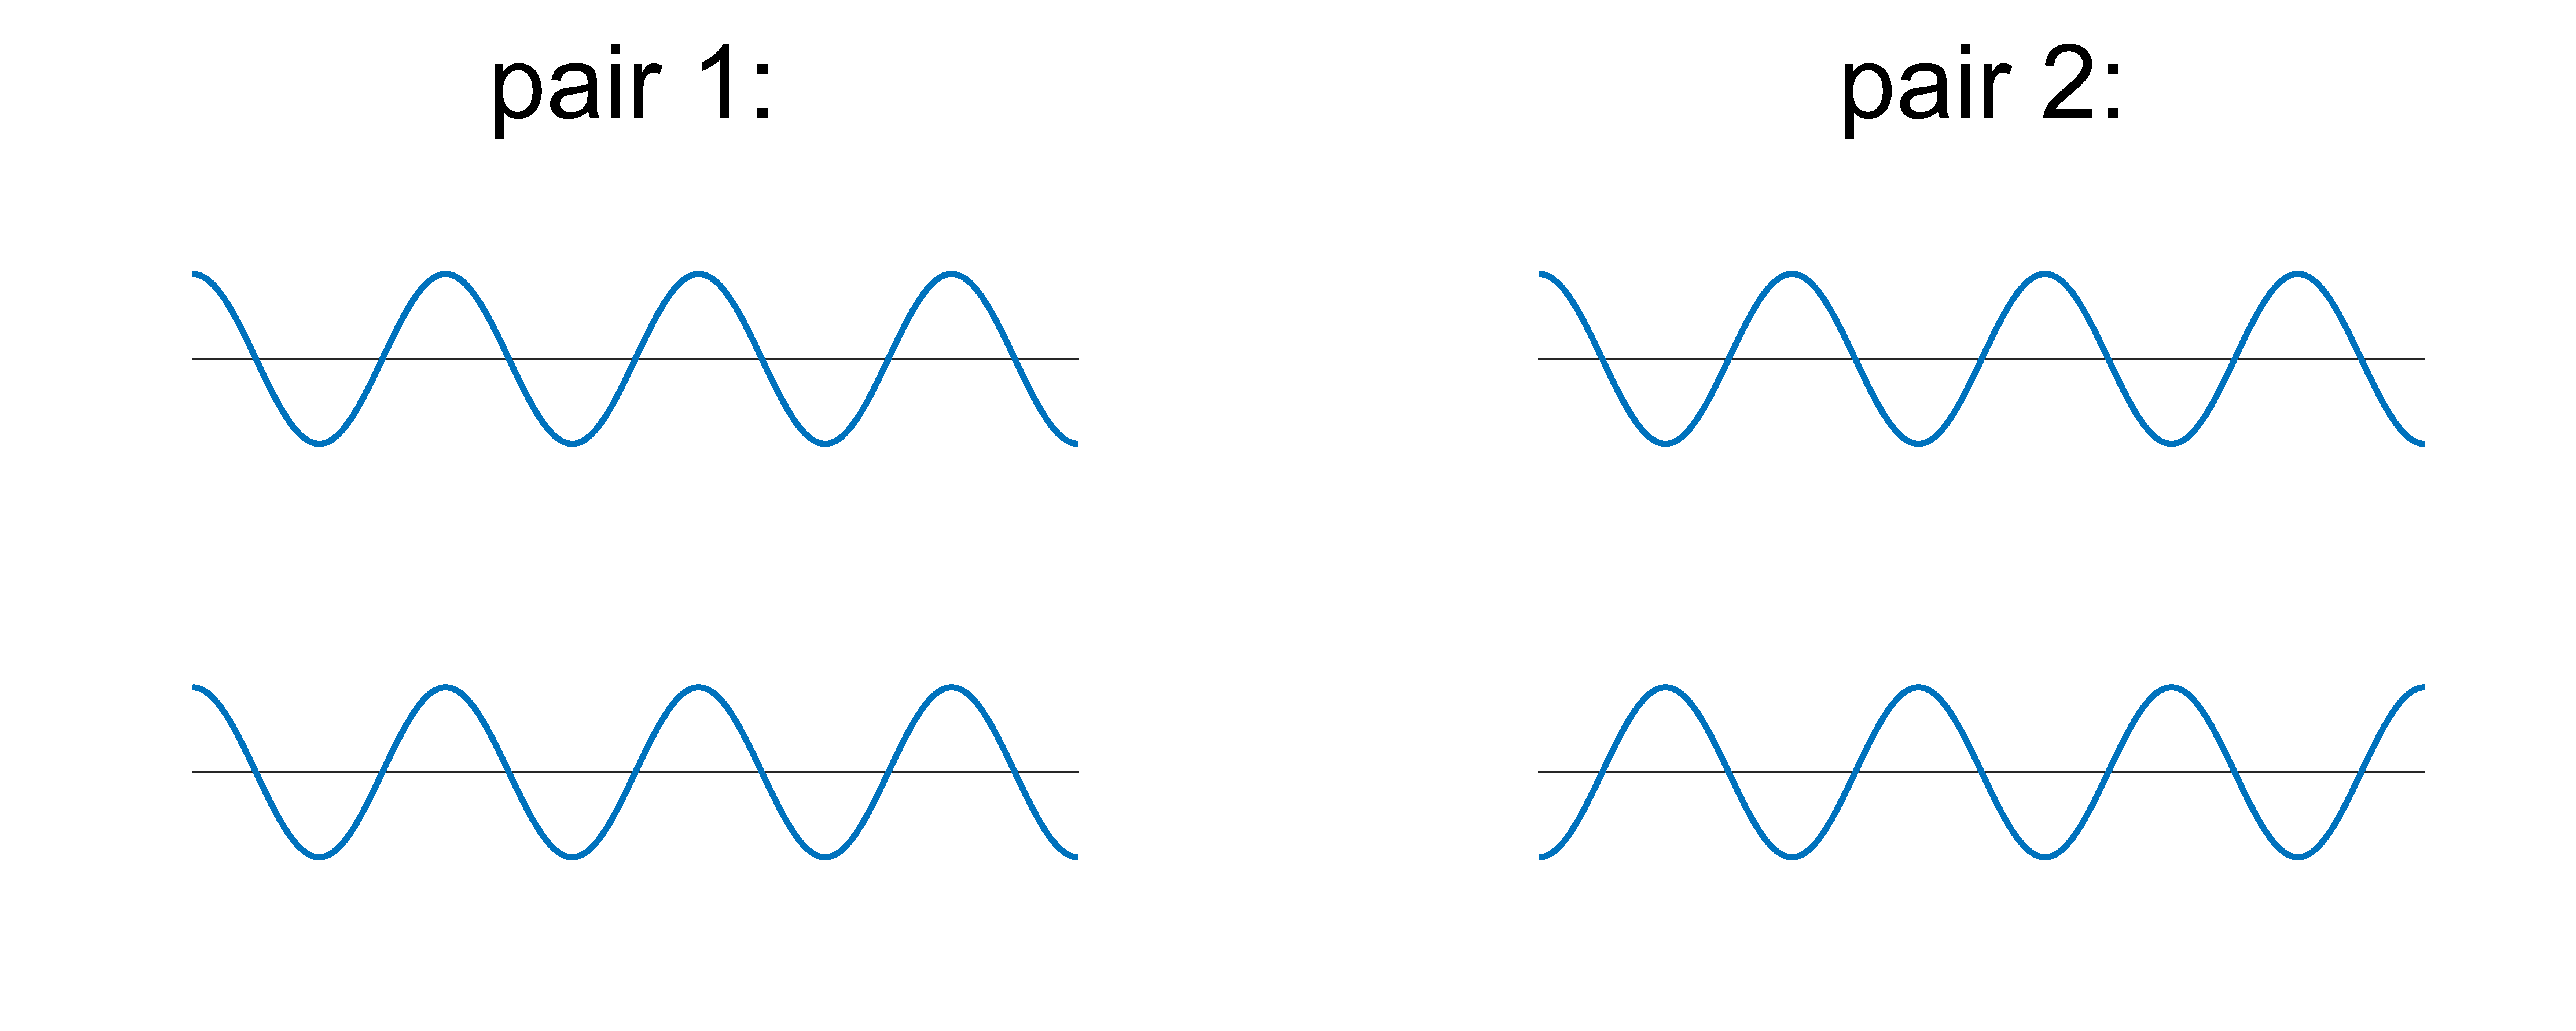
\includegraphics[width=0.7\textwidth]{\figpath/Model1_phasepairs}}
		
		Circle the pair of waves that is \emph{out} of phase.
		
	\question When two waves are travelling together, their electric fields can be \emph{added} together to obtain the total electric field at each position.
	
		Predict the total electric field as a function of the spatial position $x$ for each of the pairs of waves shown in the previous question.
		
		\begin{solution}[1in]\studentdisplay{
			\centerline{
\includegraphics[width=0.75\textwidth]{\figpath/Model1_wavesums_blank}}
		}\instructordisplay{
			\centerline{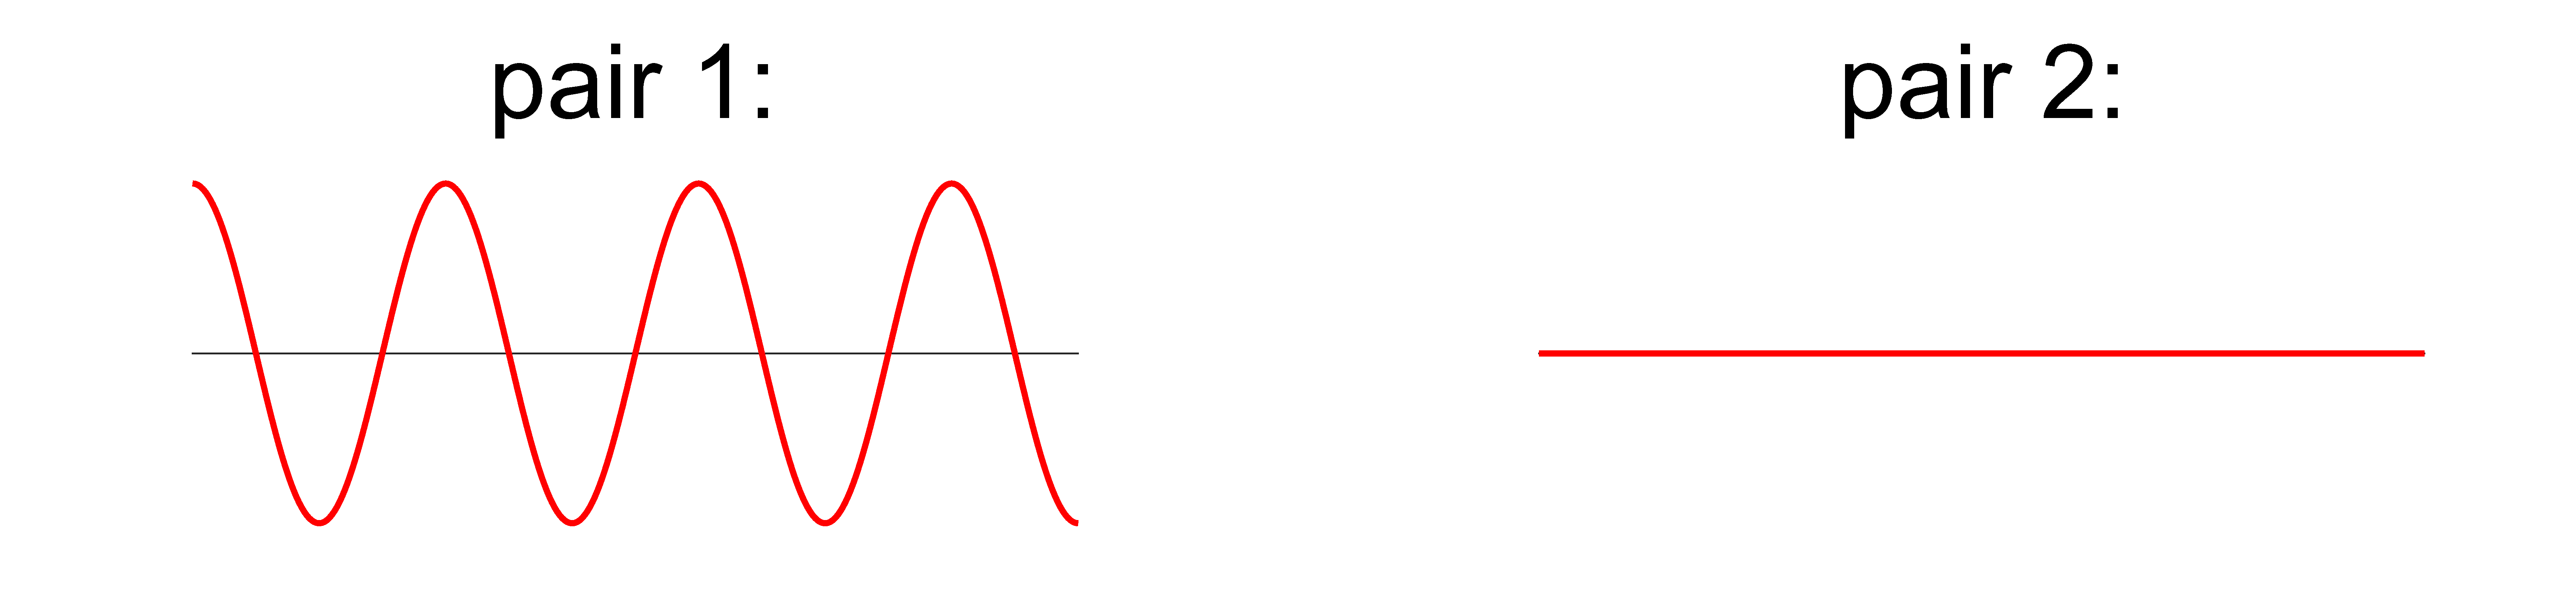
\includegraphics[width=0.7\textwidth]{\figpath/Model1_wavesums_solutions}}
		}\end{solution}
		
	\question Most detectors, including cameras and human eyes, detect only the \emph{intensity} of an electromagetic wave.  The intensity of a wave is the square magnitude of the electric field, or
	\begin{equation*}
		I = |E|^2
	\end{equation*}
	
		Based on this information, and your answer to the previous question, would you expect to detect any signal from a pair of out-of-phase waves incident on a detector?  What about from a pair of in-phase waves?  Explain your group's reasoning in 1-2 complete sentences.

\end{ctqs}

\clearpage
\begin{model}[Scattering from Multiple Particles]
\label{\labelbase:mdl:twoparticlescattering}
	
	In scattering experiments, waves originating from the same source scatter off of different particles, and take different paths to the detector.  This process is shown for waves scattering off of two particles separated by distance $d$ at angle $\theta$, below:
	
	\vspace{6pt}
	\centerline{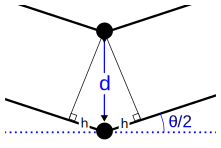
\includegraphics[width=0.8\textwidth]{\figpath/Model2_schematic}}
	
\end{model}

\begin{ctqs}

	\question As drawn, which wave travels the longer distance from the source to the detector?
	
		\begin{solution}[0.25in]
			wave 2
		\end{solution}
	
	\question As drawn, are the waves in-phase or out-of-phase when they exit the source?
	
		\begin{solution}[0.25in]
			in-phase
		\end{solution}
	
	\question As drawn, are the waves in-phase or out-of-phase when they reach the detector?
	
		\begin{solution}[0.25in]
			out-of-phase
		\end{solution}
	
	\question Explain, in 1-2 complete sentences, why the relative phase between the two waves at the detector depends on the difference in the lengths of the paths traveled by wave 1 and wave 2.
	
		\begin{solution}[1.5in]
		\end{solution}
	
	\question It is possible to show % SEE EXERCISE...
		that the difference in the path lengths of the two waves shown in Model \ref{\labelbase:mdl:twoparticlescattering} is
		\begin{equation*}
			\Delta x = 2 d \sin\left(\frac{\theta}{2}\right)
		\end{equation*}
		
		Determine whether the waves will be in-phase or out-of-phase at the detector for each of the following values of $\Delta x$:
		
		\begin{enumerate}
			\item $\Delta x = 0$:
				\begin{solution}[0.25in]
					in phase
				\end{solution}
			\item $\Delta x = \lambda/2$:
				\begin{solution}[0.25in]
					out of phase
				\end{solution}
			\item $\Delta x = \lambda$:
				\begin{solution}[0.25in]
					in phase
				\end{solution}
			\item $\Delta x = 3\lambda/2$:
				\begin{solution}[0.25in]
					out of phase
				\end{solution}
		\end{enumerate}
		
	\question Generalizing your results above, explain why the signal measured on a detector will be largest when $\Delta x = \lambda n$, where $n$ is an integer.
	
		\begin{solution}[1.5in]
		\end{solution}
	
	\question In many scattering experiments, the wavelength $\lambda$ is fixed, and the scattered intensity is measured as a function of the scattering angle, $\theta$.  Setting the equations for $\Delta x$ from the previous two questions equal to each other and rearranging, we find that the maximum signal occurs at angles
		\begin{align*}
			\sin \frac{\theta}{2} = \frac{\lambda n}{2d} && \text{or} && \theta = 2\sin^{-1}\left(\frac{\lambda n}{2d}\right)
		\end{align*}
		Mark the angles at which the maximum intensity would be measured for particles separated by each of the following distances, assuming the scattering experiment is conducted using light with a wavelength of $\lambda=500\text{ nm}$:
		
		\begin{solution}[1.5in]\studentdisplay{
			\centerline{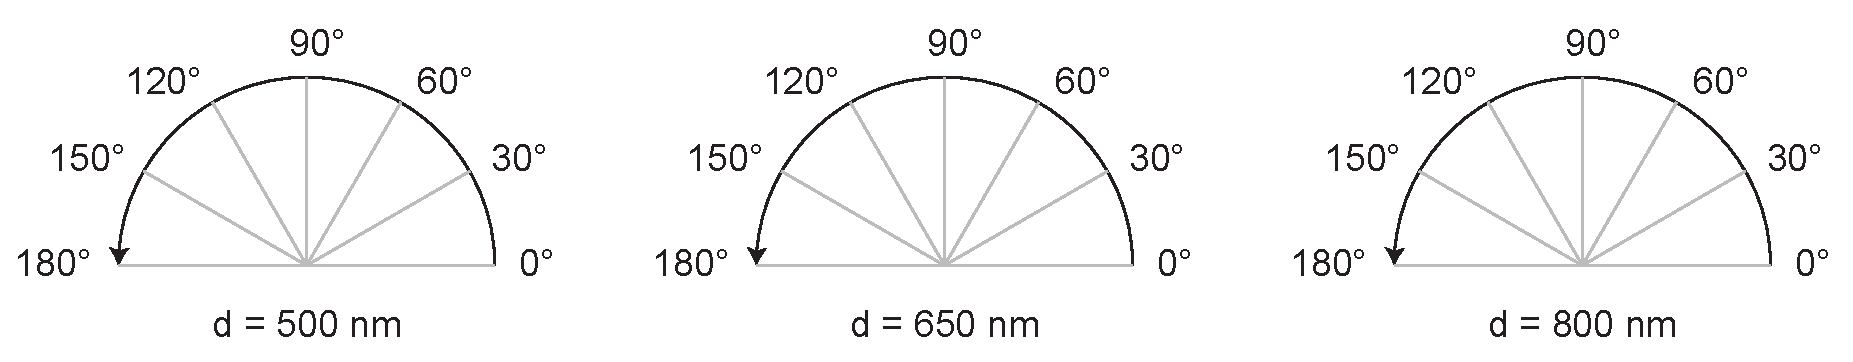
\includegraphics[width=\textwidth]{\figpath/Model2_theta_d_blank.pdf}}
		}\instructordisplay{
			\centerline{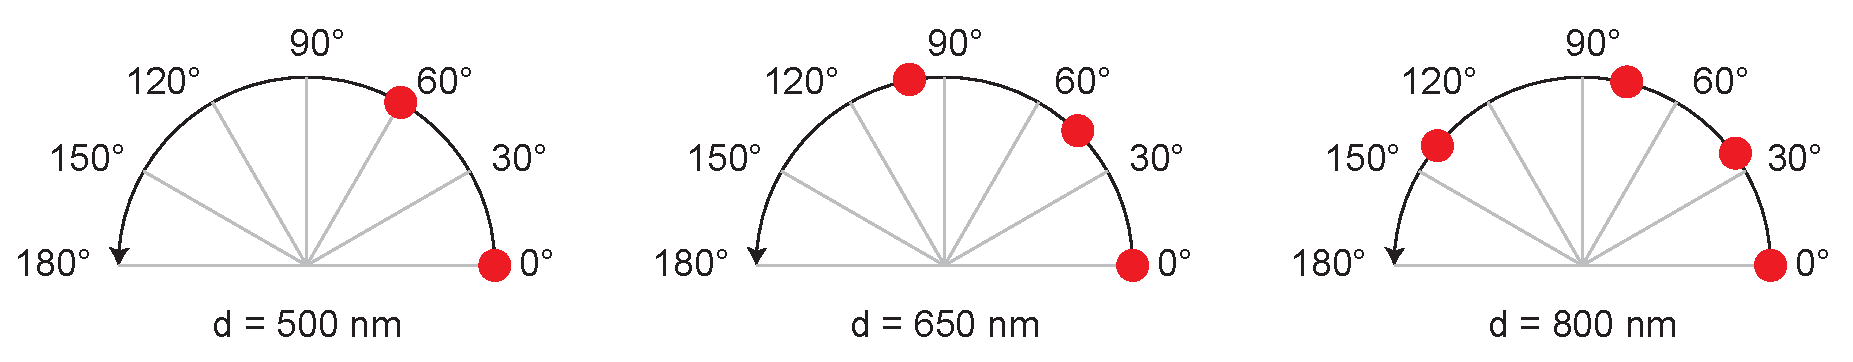
\includegraphics[width=\textwidth]{\figpath/Model2_theta_d_solutions.pdf}}
		}\end{solution}
		
	\question Explain, in 2-3 complete sentences, how scattering experiments could be used to obtain information about the distances between different particles in a sample.
	
		\begin{solution}[2in]
		\end{solution}
	
	\question Would a scattering experiment conducted using light with $\lambda=500\text{ nm}$ give useful information about the distance between the particles if $d$ were very small (say, $d=1\text{ nm}$) or very large (e.g. $d=100~\mu\text{m}$?  Explain your group's reasoning in 2-3 complete sentences.
	
		\begin{solution}[2in]
		\end{solution}
	
\end{ctqs}


\begin{infobox}%[Scattering Experiments in Polymer Science]

	Three common types of scattering experiments used in polymer science are \emph{light} scattering, \emph{X-ray} scattering, and \emph{neutron} scattering.
	
	Typical ranges of wavelengths and angles accessible in each of these types of experiment are summarized below:
	
	\begin{center}
	\renewcommand{\arraystretch}{1.3}
	\begin{tabular}{ccc}
		\hline
		\textbf{Experiment} & \textbf{Wavelength ($\lambda$)} & \textbf{Angles ($\theta$)}\\\hline
		Light Scattering & 400-700~nm & 20-160${}^\circ$ \\
		Small-Angle X-ray Scattering & 0.05-0.2~nm & 0.1-5${}^\circ$\\ 
		Wide-Angle X-ray Scattering & 0.5-1.8~\AA & 5-60${}^\circ$\\
		Small-Angle Neutron Scattering & 4-20~\AA & 0.1-3${}^\circ$\\\hline
	\end{tabular}
	\end{center}

\end{infobox}

\begin{ctqs}

	\question Which type(s) of experiment(s) would be most suitable for measuring each of the following features or processes in polymer systems?  Briefly indicate your reasoning for each item.
	
		\begin{enumerate}
		
			\item The radius of gyration of a polymer chain
			
				\begin{solution}[0.5in]
				\end{solution}
			
			\item The characteristic domain spacing of a block copolymer
			
				\begin{solution}[0.5in]
				\end{solution}
				
			\item The arrangement of atoms in a polyethylene crystal
			
				\begin{solution}[0.5in]
				\end{solution}
			
			\item The diffusion of a polymer micelle over a distance of $\sim 1~\mu$m
			
				\begin{solution}[0.5in]
				\end{solution}
			
		\end{enumerate}
	
\end{ctqs}


%\begin{exercises}

%	\exercise Sum waves that are offset by phase angles other than 0 and pi
	
%\end{exercises}


%\begin{problems}
%
%	\problem Derive the expression for $\Delta x$ in Model 2
%	
%\end{problems}


	
\end{activity}